\documentclass[12pt]{article}
\usepackage[margin=1in]{geometry} 
\usepackage{graphicx}
\usepackage{amsmath,amsthm,amssymb}
\usepackage{hyperref}

\title{
    \textbf{Theory Assignment 1} \\ 
    \textbf{CS5280} \\
}

\author{
    \textbf{Darpan Gaur} \\
    \textbf{CO21BTECH11004}
}


\date{}

\begin{document}
\maketitle

\hrulefill

\section*{Problem 1}
To show that prefix order defined on $ \Sigma^* $ is a partial order, we need to show that it is reflexive, anti-symmetric and transitive. \\
\\
(a) Reflexivity: $ (a, a) \in \Sigma^* $ \\
Let $ a \in \Sigma^* $, then $ a $ is prefix of itself. \\
$ \implies a = a $ \quad $ \implies a \preceq a $ \\
Hence, $ (a, a) \in \Sigma^* $, so relation is reflexive. \\
\\
(b) Anti-symmetry: $ (a, b) \in \Sigma^* $ and $ (b, a) \in \Sigma^* \implies a = b $ \\
Let $ a, b \in \Sigma^* $ such that $ (a, b) \in \Sigma^* $ and $ (b, a) \in \Sigma^* $ \\
$ \implies a $ is prefix of $ b $ and $ b $ is prefix of $ a $ \\
This can only happen when $ a = b $ \\
Hence, $ (a, b) \in \Sigma^* $ and $ (b, a) \in \Sigma^* \implies a = b $ \\
\\
(c) Transitivity: $ (a, b) \in \Sigma^* $ and $ (b, c) \in \Sigma^* \implies (a, c) \in \Sigma^* $ \\
Let $ a, b, c \in \Sigma^* $ such that $ a $ is prefix of $ b $ and $ b $ is prefix of $ c $ \\
$ \implies a \preceq b $ and $ b \preceq c $ \\
$ \implies a \preceq c $ \\
Hence, $ (a, b) \in \Sigma^* $ and $ (b, c) \in \Sigma^* \implies (a, c) \in \Sigma^* $ \\


\section*{Problem 2}
\begin{equation*}
    s = r_1(x) r_2(y) w_1(y) r_3(z) w_3(z) r_2(x) w_2(z) w_1(x) c_1 c_2 c_3
\end{equation*}
(a) $H[s]$
\begin{equation*}
    H[s](x) = H_s(w_1(x)) = f_{1x}(H_s(r_1(x))) = f_{1x}(H_s(w_0(x))) = f_{1x}(f_{0x}())
\end{equation*} 
\begin{equation*}
    H[s](y) = H_s(w_1(y)) = f_{1y}(H_s(r_1(x))) = f_{1y}(H_s(w_0(x))) = f_{1y}(f_{0x}())
\end{equation*}
\begin{equation*}
    \begin{split}
        H[s](z) &= H_s(w_2(z)) \\
        &= f_{2z}(H_s(r_2(x), H_s(r_2(y))))  \\ 
        &= f_{2z}(H_s(w_0(x)), H_s(w_0(y))) \\
        &= f_{2z}(f_{0x}(), f_{0y}())
    \end{split}
\end{equation*}
(b) $ RF, LRF $
\begin{equation*}
    RF(s) = \{(t_0, x, t_1), (t_0, y, t_2), (t_0, z, t_3), (t_0, x, t_2), (t_1, x, t_\infty), (t_1, y, t_\infty), (t_2, z, t_\infty)\}
\end{equation*}
\begin{equation*}
    LRF(s) = \{(t_0, x, t_1), (t_0, y, t_2), (t_0, x, t_2), (t_1, x, t_\infty), (t_1, y, t_\infty), (t_2, z, t_\infty)\}
\end{equation*}
(c) Step Graph
Find the step graph of the schedule $s$ in the figure 1.
\begin{figure}[h]
    \centering
    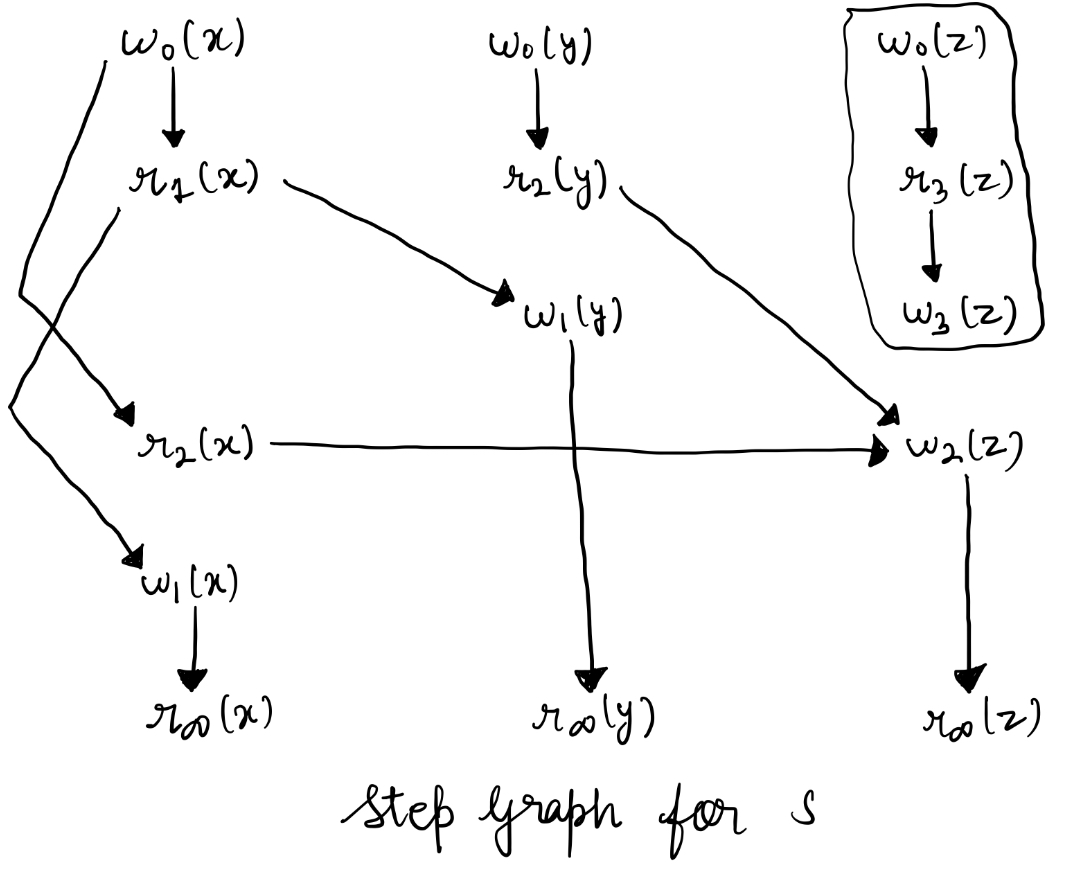
\includegraphics[width=0.75\textwidth]{images/stepGraph.jpg}
    \caption{Step Graph}
\end{figure}


\section*{Problem 3}
\begin{equation*}
    s = r_3(z) r_1(y) w_3(z) w_1(y) r_1(x) r_2(y) w_2(y) w_1(x) r_2(x) w_2(x) c_1 c_2 c_3
\end{equation*}
\begin{equation*}
    s' = r_3(z) w_3(z) r_2(y) w_2(y) r_1(y) w_1(y) r_2(x) w_2(x) r_1(x) w_1(x) c_3 c_2 c_1
\end{equation*}

(a) $H[s]$
\begin{equation*}
    \begin{split}
        H(s)[x] &= H_s(w_2(x)) \\
        &= f_{2x}(H_s(r_2(x)), H_s(r_2(y))) \\
        &= f_{2x}(H_s(w_1(x)), H_s(w_1(y))) \\
        &= f_{2x}(f_{1x}(H_s(r_1(x)), H_s(r_1(y))), f_{1y}(H_s(r_1(y))) \\
        &= f_{2x}(f_{1x}(f_{0x}(), f_{0y}()), f_{1y}(f_{0y}()))
    \end{split}
\end{equation*}
\begin{equation*}
    \begin{split}
        H(s)[y] &= H_s(w_2(y)) \\
        &= f_{2y}(H_s(r_2(y))) \\
        &= f_{2y}(H_s(w_1(y))) \\
        &= f_{2y}(f_{1y}(H_s(r_1(y)))) \\
        &= f_{2y}(f_{1y}(f_{0y}()))
    \end{split}
\end{equation*}
\begin{equation*}
    \begin{split}
        H(s)[z] &= H_s(w_3(z)) \\
        &= f_{3z}(H_s(r_3(z))) \\
        &= f_{3z}(f_{0z}())
    \end{split}
\end{equation*}

(b) $H[s']$
\begin{equation*}
    \begin{split}
        H(s)[x] &= H_s(w_1(x)) \\
        &= f_{1x}(H_s(r_1(x)), H_s(r_1(y))) \\
        &= f_{1x}(H_s(w_2(x)), H_s(w_2(y))) \\
        &= f_{1x}(f_{2x}(H_s(r_2(x)), H_s(r_2(y))), f_{2y}(H_s(r_2(y)))) \\
        &= f_{1x}(f_{2x}(f_{0x}(), f_{0y}()), f_{2y}(f_{0y}()))
    \end{split}
\end{equation*}
\begin{equation*}
    \begin{split}
        H(s)[y] = &= H_s(w_1(y)) \\
        &= f_{1y}(H_s(r_1(y))) \\
        &= f_{1y}(H_s(w_2(y))) \\
        &= f_{1y}(f_{2y}(H_s(r_2(y))) \\
        &= f_{1y}(f_{2y}(f_{0y}()))
    \end{split}
\end{equation*}
\begin{equation*}
    \begin{split}
        H(s)[z] &= H_s(w_3(z)) \\
        &= f_{3z}(H_s(r_3(z))) \\
        &= f_{3z}(f_{0z}())
    \end{split}
\end{equation*}

\end{document}